\documentclass{article}
\usepackage[ruled,linesnumbered]{algorithm2e}
\def\showtopic{Numerical Analysis}
\def\showtitle{Lab 2: Numerical Integration}
\def\showabs{Lab 2}
\def\showauthor{Ting Lin, 1700010644}
\usepackage{amsmath, amsfonts, amsthm}

\usepackage{graphicx, epstopdf}
\usepackage{color}
\usepackage{geometry, graphicx}
\usepackage{algorithm, algorithmic}
\usepackage{bm}
\usepackage{multirow}
\usepackage{ulem}
\geometry{left = 5em, right = 5em}
\usepackage{listings}
\usepackage{xcolor}
%% notation macro
\newcommand{\F}{\mathcal F}
\newcommand{\T}{\mathcal T}
\newcommand{\I}{\mathcal I}
\newcommand{\U}{\mathcal U}
\newcommand{\R}{\mathbb R}
\renewcommand{\P}{\mathcal P}
\newcommand{\uP}{ \mathcal \uline P}
\newcommand{\B}{\mathcal B}
%\newcommand{\R}{\mathbb R^2}
\newcommand{\Z}{\mathbb Z}
\newcommand{\C}{\mathbb C}
\newcommand{\laplacian}{\triangle}
\newcommand{\grad}{\nabla}
\renewcommand{\div}{\textrm{div~}}

\newcommand{\diff}[2]{\frac{\partial #1}{\partial #2}}
\newcommand{\difff}[3]{\frac{\parial #1^2}{\partial #2 \partial #3}}
\newcommand{\diFF}[2]{\frac{\partial #1^2}{\partial^2 #2}}
\newcommand{\diam}{\text{ diam }}
%% non-noation macro
\newcommand{\IN}{\text{  in  }}
\newcommand{\ON}{\text{  on  }}
\newcommand{\st}{\text{s.t.  }}
\newcommand{\tbc}{{\color{red}[TBC]}}

%% enviorment
\newtheorem{proposition}{Proposition}
\newtheorem{definition}{Definition}
\newtheorem{corollary}{Corollary}
\newtheorem{remark}{Remark}



\title{\textbf{\showtitle}}
\author{\showauthor}
\usepackage{indentfirst}
\usepackage{fancyhdr}  
\pagestyle{fancy}
\lhead{\textbf {\showtopic} }
\chead{} 
\rhead{\textbf {\showabs} }
\lfoot{} 
\cfoot{\thepage}
\rfoot{} 
\renewcommand{\headrulewidth}{0.4pt} 

\newcommand{\return}{\textbf{return~}}
\begin{document}
	\maketitle
	\thispagestyle{fancy}
	\tableofcontents
	
	\section*{}
In this section we introduce two kind of numerical integration formula, Cotes formula and Gauss formula. For practical use, we introduce composite integration method and adaptive integration method. We will show their difference by numerical example 



\section{Numerical Integration Formula}
\subsection{Interpolation Type and Algebraic Precision}
We mainly discuss numerical of\textbf{ interpolation type}: for a given interval $[a,b]$ and $f \in C[a,b]$, the numerical interpolation respect to a node set $\Delta: x_0 < \cdots x_k  \in [a,b]$ is defined as 
$$I_N(f) = \int_{a}^b P_{\Delta}f$$
where $P_{\Delta}f \in \mathcal P_{k}$ is the polynomial interpolation of $f$. An equivalent definition is that $I(f) = \sum_{k=0}^n A_kf(x_k)$ satisfies that $I_N(f) = I(f):=\int_{a}^{b} f(x) $ for all polynomials with degree $\le n$. The equivalence is proved in [CITE]. 

For a given node set $\Delta$, suppose the interpolation operator $P_{\Delta}f = \sum_{k=0}^n l_k(x)f(x_k)$, then $A_k = \int_a^b l_k(x) dx$. 
To describe the error of a given numerical formula $\tilde I$, we introduce the definition of algebraic precision. 

\begin{definition}
	If $\tilde I (f) = I(f)$ for all polynomials $f$ with degree $\le m$, but fails for higher degree, we say that the numerical formula is of \textbf{$m$-th order algebraic precision}, or briefly $m$-th order if there is no ambiguity.
\end{definition}

Clearly if $I_n$ is of interpolation type, then it must be at least $n$-th order, the converse is also true from the equivalent definition. The further result is statemented below.
\begin{proposition}
	For $0\le k \le n+1$, $I_N(f)$ is $k+d$-th order if and only if 
	\begin{enumerate}
		\item $I_N$ is of interpolation type, respect to some node set $x_0<\cdots, x_n \in [a,b]$.
		\item $\omega(x) = \prod_{i=0}^n (x-x_i)$ is orthogonal to $\mathcal P_{k-1}$.
	\end{enumerate}
\end{proposition}

\subsection{Newton--Cotes formula and Gauss formula}
We introduce two types of integration formula, under the aforementioned framework. If we choose the node set being $\Delta^{NC} : a, a+\frac{h}{n-1}, a+\frac{2h}{n-1}, \cdots a + h=b$, where $h = b-a$, then we derive the Newton--Cotes formula:
$$I_N^{NC}(f) = \sum_{k=0}^{n} A_k f(x_k),$$
where $x_k = a + \frac{kh}{n-1}$. 
Direct observation on $\int_a^b \omega(x)$ we have the following proposition.

\begin{proposition}
	If $n$ is odd, then $I_N^{NC}$ is $n$-th order. If $n$ is even, the it is $n+1$-th order.
\end{proposition}

To seek a formula with higher order, one should recall the Legendre polynomial $L_n(a,b)$, which is orthogonal to $\mathcal P$ automatically. Hence if we choose the node set $\Delta$ being the roots of $L_n$, by the proposition we will obtain at least $(n-1) + n =2n-1$-th order. (Notice that $L_n(a,b)$ has only $n$ distinct real roots). We derive the Gauss formula:
$$I_N^{G}(f) = \sum_{k=1}^{n} A_k f(x_k),$$
where $x_k$ are the roots of $L_n(a,b)$. Since $I(L_k^2)\neq 0 = I_N^G(L_k^2)$, the Gauss formula is exactly $(2n-1)$-th order.

By considering an affine transform $[a,b] \to [0,1]$, we can easily represent the formula discussed above as
$$I_N(f) = (b-a)\sum_{k = 1}^{n} w_kf(a + (b-a)c_k).$$ Here $w_k$ and $c_k$ are independent to $[a,b]$. In practical implementation, we use two arrays to store the value of $w_k$ and $c_k$, yielding the following algorithm.

\begin{algorithm}
	\caption{Simple-Int}
\KwIn{$f, w, c,a,b$}
\KwOut{$I$}
$I = 0, ~~ h = b-a$
\For{$i = 0:length(c)$}{$I = I + h*w[i]f(a+h*c[i]))$}
\return I
\end{algorithm}


\subsection{Composite Integration and Adaptive Integration}
Composite integration is to use the simple integration formula, introduce in the previous subsection, into the sub-interval, and sum the result up.
\begin{algorithm}
	\caption{Composite-Int}
	\DontPrintSemicolon
	\KwIn{$f, a,b,M,w,c$ \tcc*{$M$ is the number of sub-interval}} 
	\KwOut{$I$}
	$I = 0$
	
	$h = (b-a)/M$
	\For{$i = 0:M-1$}{Calculate $I_i = \textbf{Simple-Int}(f,w,c,a+ih, a+(i+1)h)$
	
$I = I + I_i$}

\return $I$
	
\end{algorithm}

For the composite integration formula, we have the following estimates:
\begin{proposition}
	If the integration formula is of $k$, then we have $$|I_N(f) - I(f)| \le Ch^{k+1}.$$
\end{proposition}
A more wiser choice is to use the adaptive integration, for a given tolerance $tol$(typically $1e-12$ or $1e-16$), we introduce the following algorithm. 
\begin{algorithm}
	\caption{Adaptive-Int}
	\KwIn{$f,a,b,w,c$}
	\KwOut{$I$}
	$m = \frac{a+b}{2}$
	
	\eIf{ $|\textbf{Simple-Int}(f,w,c,a, m) + \textbf{Simple-Int}(f,w,c,m, b) - \textbf{Simple-Int}(f,w,c,a, b)| \le (b-a)tol$}{\return $\textbf{Simple-Int}(f,w,c,a, b)$}{\return $\textbf{Adaptive-Int}(f,w,c,a, m) + \textbf{Adaptive-Int}(f,w,c,m, b)$}
\end{algorithm}
\section{Question}
In this report we focus on the integral
$$F = \int_{0}^{\infty}\frac{x^3}{e^x-1}dx.$$
Clearly, $F$ is finite, but it is integrated on a infinite interval. Hence we need to do some preprocessing. (Notice if we want to obtain a more accuracy one, we will not adopt the Gauss-Laguerre interpolation)

\subsection{Preprocessing}
First, rather than computing $F$, we compute 
$$G = \int_{0}^{\infty} \frac{x^3}{(e^x-1)e^x} dx$$ instead. Since $$F - G = \int_{0}^{\infty} x^3e^{-x} dx = \Gamma(3) = 6.$$
A reason that we prefer computing $G$ is that $G$ is decaying more rapidly than $F$, thus we can use a small $M$ to truncate, that is, using 
$$\tilde G = \int_{0}^{30}\frac{x^3}{(e^x-1)e^x} dx$$ instead of $G$. We first show the error estimates.

\begin{proposition}
	$$\int_{30}^{\infty}\frac{x^3}{(e^x-1)e^x} dx < 10^{-16}$$
\end{proposition}
\begin{proof}
	\begin{equation*}
	\begin{split}
	\int_{30}^{\infty}\frac{x^3}{(e^x-1)e^x} dx  &< \frac{1}{e^{30}-1}\int_{30}^{\infty}x^3e^{-x}dx \\
	& < \frac{1}{e^{30}-1}*\int_{30}^{\infty}\frac{(12)!x^3}{x^{12}} dx\\
	& < \frac{1}{e^{30}-1}\frac{(12)!}{8(30)^8}\\
	& < 10^{-16}
	\end{split}
	\end{equation*}
\end{proof}

\subsection{Numerical Result and Discussion}
We first test the composite integration and adaptive integration (with $tol = 1e-16$).
\begin{table}[H]
	\begin{tabular}{|l|l|l|l|l|l|l|l|}
		\hline
		& 50        & 100       & order & 200       & order & adaptive node & adaptive result    \\ \hline
		Trapezoid(Cotes1) & 1.53E-03  & 9.98E-05  & 3.93  & 6.31E-06  & 3.98  & -             & -                  \\ \hline
		Simpson(Cotes2)   & 3.77E-04 & 2.49E-05 & 3.92  & 1.57E-06 & 3.98  & 9224          & 0.49393940226683   \\ \hline
		Cotes3            & 1.69E-04 & 1.11E-05 & 3.93  &7.00E-07 & 3.98  & 7658          & 0.493939402266829  \\ \hline
		Cotes4            & 1.39E-06 & 2.24E-08 & 5.95  & 3.52E-10 & 5.98  & 446           & 0.4939394022668297 \\ \hline
		Midpoint(Gauss1)  & 1.33E-03 & 8.72E-05 & 3.93  & 5.52E-06 & 3.98  & -             & -                  \\ \hline
		Gauss2            & 2.50E-04  & 1.66E-05  & 3.91  & 1.05E-06  & 3.98  & 8429          & 0.4939394022668284 \\ \hline
		Gauss3            & 1.33E-06  & 2.15E-08  & 5.95  & 3.38E-10  & 5.99  & 443           & 0.4939394022668287 \\ \hline
	\end{tabular}
\end{table}

We also test 
There are two orders violates the theoretical result, the Trapezoid and Midpoint. First we should notice that it does not hold in general. For example, if we try to calculate $\int_0^4 \frac{x^3}{e^x-1}dx$ we obtain the following result, which shows the theoretical result is still convincing.
\begin{figure}[H]
	\centering
	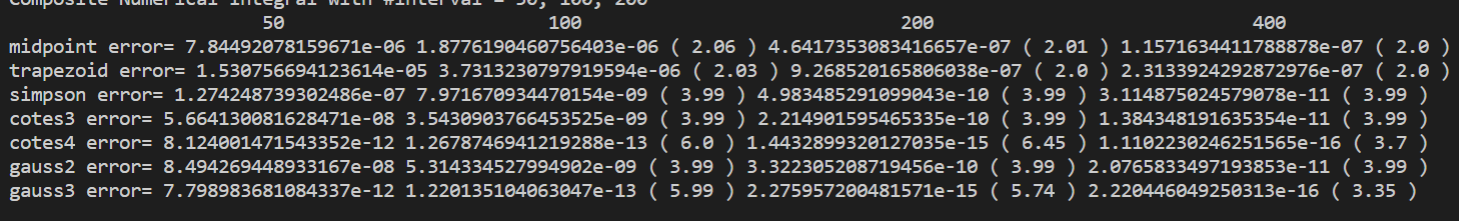
\includegraphics[scale=.5]{fig1.png}
\end{figure}

We try to change $x^3$ to $x^2$, obtaining the following result. 
$$I = \int_{0}^{30}\frac{x^2}{e^x-1}dx$$
\begin{figure}[H]
	\centering
	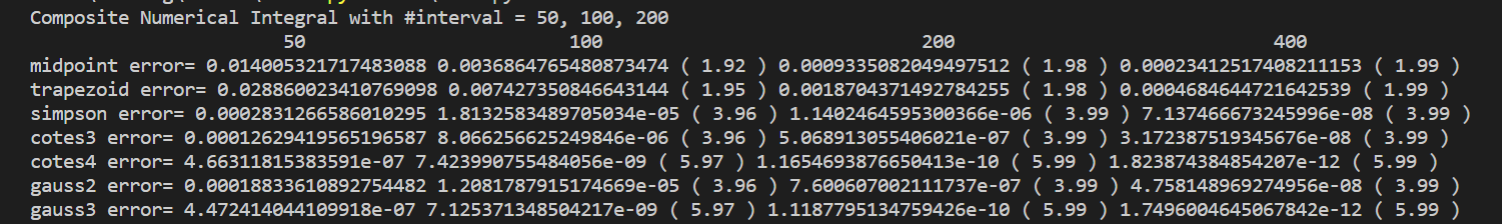
\includegraphics[scale=.5]{fig2.png}
\end{figure}

We give a proper explanation for this phenomenon.
\begin{proposition}
	For composite integration method with midpoint (trapezoid) integrator as an inner routine, it holds
	\begin{equation}
	|I_N^h(f)-I(f)|=\mathcal O (h^4)
	\end{equation}
	if $\int_a^b f''(x)\,dx=0$.
\end{proposition}
\begin{proof}
	Assume $b-a=nh$. For midpoint rule, denote the middle point of each sub-interval as $c_j=a+(j+\frac{1}{2})h$. By Taylor expansion at $b_j$,
	\begin{equation}
	f(x)=f(c_j)+(x-c_j)f'(c_j)+\frac{(x-c_j)^2}{2}f''(c_j)+\frac{(x-c_j)^3}{6}f'''(c_j) +\mathcal O (h^4),
	\end{equation}
	\begin{equation}
	\begin{aligned}
	\int_{a+jh}^{a+(j+1)h} f(x)\,dx& = hf(c_j)+\frac{h^3}{24}f''(c_j)+\mathcal O(h^4)\\
	&= hf(c_j)+\frac{h^2}{24}\int_{a+jh}^{a+(j+1)h}f''(x)\,dx+\mathcal O(h^4).
	\end{aligned}
	\end{equation}
	Thus the error estimate of composite method $I_N(f)$ reads
	\begin{equation}
	\begin{aligned}
	I(f)-I_N(f) &= \int_a^b f(x)\,dx-\sum_{j=0}^{n-1} hf(c_j)\\
	&= \int_a^b f''(x)\,dx +\mathcal O(h^4)\\
	&= \mathcal O(h^4).
	\end{aligned}
	\end{equation}
	
	As to trapezoid rule, applying the result derived above to the interval $[b_0,b_{n-1}]$ yields
	\begin{equation}
	\begin{aligned}
	\int_{c_0}^{c_{n-1}}f(x)\,dx &= \sum_{j=1}^{n-1} hf(a+jh)+\int_{c_0}^{c_{n-1}}f''(x)\,dx+\mathcal O(h^4),\\ 
	\int_{a}^{c_0}f(x)\,dx+\int_{c_{n-1}}^bf(x)\,dx &= \frac{h}{2}(f(a)+f(b))+\int_a^{c_0}(x-a)f'(a)\,dx+\int_{c_{n-1}}^b (x-b)f'(b)\,dx \\ &+\frac{h^2}{24}(\int_{a}^{c_0}f''(x)\,dx+\int_{c_{n-1}}^bf''(x)\,dx)+\mathcal O(h^4)\\
	&=\frac{h}{2}(f(a)+f(b))+\frac{h^2}{24}(\int_{a}^{c_0}f''(x)\,dx+\int_{c_{n-1}}^bf''(x)\,dx)+\mathcal O(h^4),\\
	I(f)-I_N(f) &= \int_a^b f(x)\,dx-\sum_{j=1}^{n-1} hf(a+jh)-\frac{h}{2}(f(a)+f(b))\\
	&= \int_a^b f''(x)\,dx +\mathcal O(h^4)\\
	&= \mathcal O(h^4).
	\end{aligned}
	\end{equation}
\end{proof}
\subsection{Romberg Technique}
Also we can utilize the Romberg technique to obtain higher order. Suppose the method has order $k$, we then write $$I_{N,h}(f) = I(f) + C_{k}h^k + C_{k+1}h^{k+1} + C_{k+2}h^{k+2} + \cdots$$
Then simple calculation shows that 
$$I_{N,h}^R(f) = (2^kI_{N,h/2}(f) - I_{N,h}(f))/(2^k - 1)$$ is a approximation of at least $k+1$ order. Moreover, if $C_{k+1}=0$ then the scheme is of $k+2$ order.
We test the idea in numeric, see the figure below, that is exactly we desired.
\begin{figure}[H]
	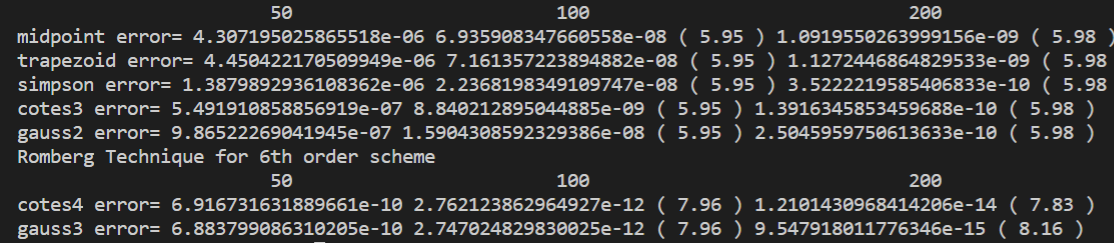
\includegraphics[scale=.4]{fig3.png}
\end{figure}


\subsection{Conclusion}
In this lab we test several integration formula in solving a simple question. We show the composite integration, Romberg technique and adaptive integration. Rather than believing the conservative estimation, we show the error and order numerically. Also we observe that in some special cases, the order will be lifted in 2-orders (like what we see in trapezoid and midpoint scheme). Also, we found that the adaptive integration is practical. 
\end{document}
















Escape special TeX symbols (%, &, _, #, $)